%%%%%%%%%%%%%%%%%%%%%%%%%%%%%%%%%%%%%%%%%
% Structured General Purpose Assignment
% LaTeX Template
%
% This template has been downloaded from:
% http://www.latextemplates.com
%
% Original author:
% Ted Pavlic (http://www.tedpavlic.com)
%
% Note:
% The \lipsum[#] commands throughout this template generate dummy text
% to fill the template out. These commands should all be removed when 
% writing assignment content.
%
%%%%%%%%%%%%%%%%%%%%%%%%%%%%%%%%%%%%%%%%%

%----------------------------------------------------------------------------------------
%	PACKAGES AND OTHER DOCUMENT CONFIGURATIONS
%----------------------------------------------------------------------------------------

\documentclass{article}

\usepackage{listings}
\usepackage{mathtools}
\usepackage{fancyhdr} % Required for custom headers
\usepackage{lastpage} % Required to determine the last page for the footer
\usepackage{extramarks} % Required for headers and footers
\usepackage{graphicx} % Required to insert images
\usepackage{lipsum} % Used for inserting dummy 'Lorem ipsum' text into the template

% Margins
\topmargin=-0.45in
\evensidemargin=0in
\oddsidemargin=0in
\textwidth=6.5in
\textheight=9.0in
\headsep=0.25in 

\linespread{1.1} % Line spacing

% Set up the header and footer
\pagestyle{fancy}
\lhead{\hmwkAuthorName} % Top left header
\chead{\hmwkClass\ (\hmwkClassInstructor\ \hmwkClassTime): \hmwkTitle} % Top center header
\rhead{\firstxmark} % Top right header
\lfoot{\lastxmark} % Bottom left footer
\cfoot{} % Bottom center footer
\rfoot{Page\ \thepage\ of\ \pageref{LastPage}} % Bottom right footer
\renewcommand\headrulewidth{0.4pt} % Size of the header rule
\renewcommand\footrulewidth{0.4pt} % Size of the footer rule

\setlength\parindent{0pt} % Removes all indentation from paragraphs

%----------------------------------------------------------------------------------------
%	DOCUMENT STRUCTURE COMMANDS
%	Skip this unless you know what you're doing
%----------------------------------------------------------------------------------------

% Header and footer for when a page split occurs within a problem environment
\newcommand{\enterProblemHeader}[1]{
\nobreak\extramarks{#1}{#1 continued on next page\ldots}\nobreak
\nobreak\extramarks{#1 (continued)}{#1 continued on next page\ldots}\nobreak
}

% Header and footer for when a page split occurs between problem environments
\newcommand{\exitProblemHeader}[1]{
\nobreak\extramarks{#1 (continued)}{#1 continued on next page\ldots}\nobreak
\nobreak\extramarks{#1}{}\nobreak
}

\setcounter{secnumdepth}{0} % Removes default section numbers
\newcounter{homeworkProblemCounter} % Creates a counter to keep track of the number of problems

\newcommand{\homeworkProblemName}{}
\newenvironment{homeworkProblem}[1][Problem \arabic{homeworkProblemCounter}]{ % Makes a new environment called homeworkProblem which takes 1 argument (custom name) but the default is "Problem #"
\stepcounter{homeworkProblemCounter} % Increase counter for number of problems
\renewcommand{\homeworkProblemName}{#1} % Assign \homeworkProblemName the name of the problem
\section{\homeworkProblemName} % Make a section in the document with the custom problem count
\enterProblemHeader{\homeworkProblemName} % Header and footer within the environment
}{
\exitProblemHeader{\homeworkProblemName} % Header and footer after the environment
}

\newcommand{\problemAnswer}[1]{ % Defines the problem answer command with the content as the only argument
\noindent\framebox[\columnwidth][c]{\begin{minipage}{0.98\columnwidth}#1\end{minipage}} % Makes the box around the problem answer and puts the content inside
}

\newcommand{\homeworkSectionName}{}
\newenvironment{homeworkSection}[1]{ % New environment for sections within homework problems, takes 1 argument - the name of the section
\renewcommand{\homeworkSectionName}{#1} % Assign \homeworkSectionName to the name of the section from the environment argument
\subsection{\homeworkSectionName} % Make a subsection with the custom name of the subsection
\enterProblemHeader{\homeworkProblemName\ [\homeworkSectionName]} % Header and footer within the environment
}{
\enterProblemHeader{\homeworkProblemName} % Header and footer after the environment
}
   
%----------------------------------------------------------------------------------------
%	NAME AND CLASS SECTION
%----------------------------------------------------------------------------------------

\newcommand{\hmwkTitle}{Project\ \#1} % Assignment title
\newcommand{\hmwkDueDate}{Tuesday,\ February\ 10,\ 2015} % Due date
\newcommand{\hmwkClass}{CSCI\ 8810} % Course/class
\newcommand{\hmwkClassTime}{08:00am} % Class/lecture time
\newcommand{\hmwkClassInstructor}{Dr. Arabnia} % Teacher/lecturer
\newcommand{\hmwkAuthorName}{Sina Solaimanpour} % Your name

%----------------------------------------------------------------------------------------
%	TITLE PAGE
%----------------------------------------------------------------------------------------

\title{
\vspace{2in}
\textmd{\textbf{\hmwkClass:\ \hmwkTitle}}\\
\normalsize\vspace{0.1in}\small{Due\ on\ \hmwkDueDate}\\
\vspace{0.1in}\large{\textit{\hmwkClassInstructor\ \hmwkClassTime}}
\vspace{3in}
}

\author{\textbf{\hmwkAuthorName}}
\date{} % Insert date here if you want it to appear below your name

%----------------------------------------------------------------------------------------

\begin{document}

\maketitle

%----------------------------------------------------------------------------------------
%	TABLE OF CONTENTS
%----------------------------------------------------------------------------------------

%\setcounter{tocdepth}{1} % Uncomment this line if you don't want subsections listed in the ToC

\newpage
\tableofcontents
\newpage

%----------------------------------------------------------------------------------------
%	Introduction
%----------------------------------------------------------------------------------------

% To have just one problem per page, simply put a \clearpage after each problem

\begin{homeworkProblem}[\Roman{homeworkProblemCounter}. Introduction to \textit{"ColonD Image Processing"}]
This project is aimed to get us more familiar with different Image Processing techniques. The overall work flow of this project is to read an image from an image source (here, the image source can be either a JPEG file or the computer's camera) and apply different image processing algorithms in the image separately and in combination.


I am using C++ programming language along with OpenCV library to implement the algorithms in this project. I chose C++ over other programming languages because of its superior performance and less overhead comparing to other high-level programming language like Java or Python. Furthermore, I am using OpenCV just to read/write images from/to a file and also to maintain the image structure in the system. All other operations are implemented without any use of existing functions.

In this phase of the project, the following features have been implemented which will be discussed in more detail in the following sections:

\begin{itemize} \itemsep1pt \parskip0pt \parsep0pt
  \item Read an image from the filesystem
  \item Capture an image from the computer's camera
  \item Create the image histogram and maintain it after each change
  \item Enhance the image contrast using image histogram
  \item Convert an image to a gray scale image
  \item Add artificially created noise to the image
  \item Smooth an image using "Average Filters"
  \item Smooth an image using "Median Filters"
  \item Convert an image to binary by simple thresholding 
  \item Image slice thresholding an image
  \item Iterative thresholding an image
  \item Adaptive thresholding an image
  \item P-tile thresholding an image
\end{itemize}

These features are all implemented and tested with different images, individually and in combination of other operations. In the next sections, I will go over each one of these features in more detail and will present some results from the program.
\end{homeworkProblem}

%----------------------------------------------------------------------------------------
%	Basic operations
%----------------------------------------------------------------------------------------

\begin{homeworkProblem}[\Roman{homeworkProblemCounter}. Basic operations]
In this section, I will go over some of the basic operations implemented in the project. These operations are:

\begin{enumerate} \itemsep1pt \parskip0pt \parsep0pt
  \item Read/Write an image from/to the filesystem
  \item Capture an image from the computer's camera
\end{enumerate}

\begin{homeworkSection}{(a) Read/Write operations} % Section within problem

For these two operations, I am using OpenCV's imread and imwrite functions. The imread function will read an image file and load it into a Mat data structure which is the image structure in OpenCV. On the other hand, the imwrite function will get as parameter a Mat object and will serialize it to the filesystem.

I faced some difficulties using these two functions. An example of these difficulties was the incompatibilities between color spaces. The imread function reads an image in BGR color space and I was processing the image in RGB space. This forced me to convert the read images to RGB, after reading it and, convert them back to BGR before writing to the filesystem.

\end{homeworkSection}

\begin{homeworkSection}{(b) Capture image from camera} % Section within problem

As an extra feature, I added the capture image functionality to the program. To do this, I get the system's default camera and open its video feedback in a different window. The user can hit the "Space" key to capture the image. After that, the captured image will be opened in the program automatically and it can be used as a normal image in the program.

Again, this image capturing process had the exact same problem with the color spaces as Read/Write operations. I have applied the color space conversion in this context too.

\end{homeworkSection}

\end{homeworkProblem}

%----------------------------------------------------------------------------------------
%	Histogram
%----------------------------------------------------------------------------------------

\begin{homeworkProblem}[\Roman{homeworkProblemCounter}. Histogram view]
After opening or capturing an image in the program, a new window will appear which is consisted of the histogram of the image. For simplification, I have used the red channel to create and show the histogram and this will allow us to show almost the same histograms for both an color image and the gray scale version of it. This could be done by creating four different histograms, one for each RGB channels and one for the average of the three values.

To create the histogram chart, I have used GNU-Plot program installed on an UBUNTU machine. Each time the image changes, I will update its histogram and send it over to GNU-plot to create the chart. Then, I use the created histogram to update the Histogram view in the program.

\begin{figure}[h!]
  \centering
    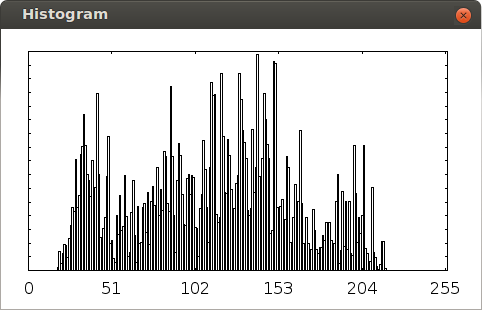
\includegraphics[width=0.5\textwidth]{histogram}
  \caption{Screen shot of a sample histogram created in the program.}
\end{figure}

\end{homeworkProblem}

%----------------------------------------------------------------------------------------
%	Gray Scale
%----------------------------------------------------------------------------------------

\begin{homeworkProblem}[\Roman{homeworkProblemCounter}. Gray Scale Conversion]
As we are supposed to process only gray scale images, I needed to somehow convert the read image to gray scale. I tried three different methods to convert the color image to gray scale image. After comparing the results from different techniques on multiple images, I decided to use the weighted average as the main algorithm to convert the images to gray scale in my program. The following equation is used to get the resulting gray scale pixels in the image.

\lstset {language=C++}
\begin{lstlisting}
int gray_scale = 0.21 * red + 0.72 * green + 0.07 * blue;
\end{lstlisting}

Also, the following image is the result from converting the original version of the Lena image to gray scale using the ColonD program.

\begin{figure}[h!]
  \centering
    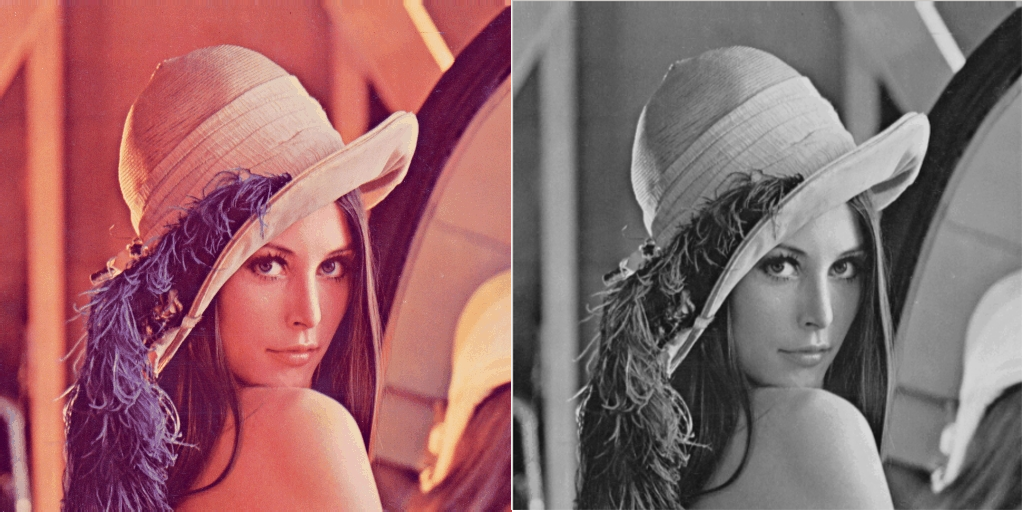
\includegraphics[width=0.6\textwidth]{grayscale}
  \caption{Convert lena's image to gray scale.}
\end{figure}

\end{homeworkProblem}

%----------------------------------------------------------------------------------------
%	Noise
%----------------------------------------------------------------------------------------

\begin{homeworkProblem}[\Roman{homeworkProblemCounter}. Add Noise]

For learning purposes, we needed to add some artificially created noise to our images. In my project, using a slider control, one can add different amounts of noise to the opened image. The implementation of this feature was very simple but again, it could be done in different ways. What I am doing is, I get a totally random number in \textit{P} percent of the pixels and replace the pixel value with the random number. Another way of doing this is to generate a random number and add the random value to the pixel values.

The user can use the slider to change the amount of added noise to the picture and by clicking on the "Apply" button the noise will be added to the image. If one forgets to click on the apply button to decide not to add noise to the image, the noise will not be applied and the original image will remain intact.

\begin{figure}[h!]
  \centering
    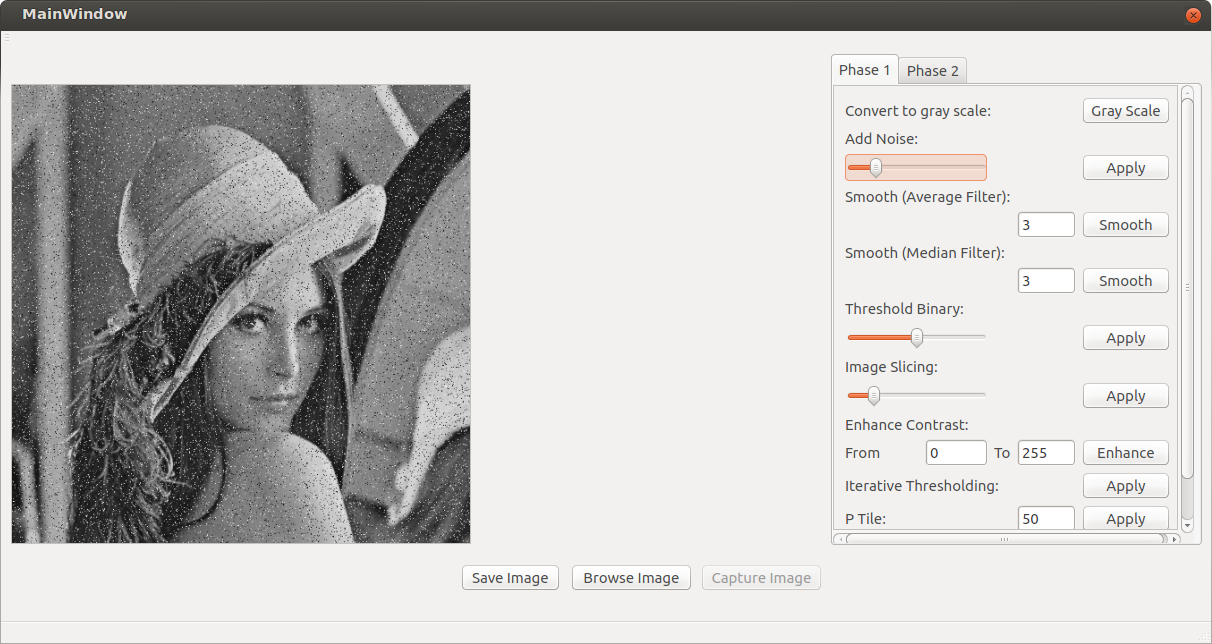
\includegraphics[width=0.75\textwidth]{noise}
  \caption{Added some noise to the lena's picture. The slider control and the Apply button can be seen in this snapshot of the program.}
\end{figure}

\end{homeworkProblem}

%----------------------------------------------------------------------------------------
%	Smoothing
%----------------------------------------------------------------------------------------

\begin{homeworkProblem}[\Roman{homeworkProblemCounter}. Add Noise]

For smoothing an image, we can use two different techniques in this program. These two techniques will be explained in detail in the following sub-sections.


\begin{homeworkSection}{(a) Average Filter} % Section within problem

This technique is nothing but using a simple filter over the image. The matrix which represents the filter have equal values as for each one its elements and this value is equal to $\frac{1}{Width ^ 2}$.

The user can use the provided textfields to determine the width of the filter. The following figure will depict how the Average Filtering algorithm will work on an image.

\begin{figure}[h!]
  \centering
    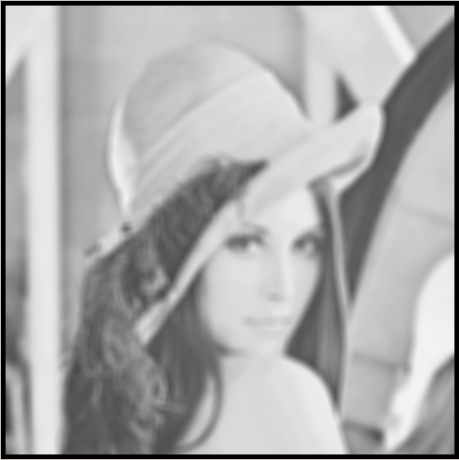
\includegraphics[width=0.3\textwidth]{average}
  \caption{Used an Average Filter with Width = 10 on lena's image.}
\end{figure}

This algorithm will leave out a few pixels from each side of the image and will not fill them with any other values hence the black frame around the image is formed.

\end{homeworkSection}

\begin{homeworkSection}{(b) Median Filter} % Section within problem

This filter will find the pixel values in corresponding to the filter elements, sort them and use the middle value (the median) to represent all other pixels as well for the pixel corresponding to the filter's middle element.

I realized that this smoothing technique will work very well on noisy images I created using the Add Noise feature. The following figure will compare both the noisy and the smoothed image together. As you can see, the resulting smoothed image has a huge improved \textbf{visual quality}  comparing to the noisy image.

\begin{figure}[h!]
  \centering
    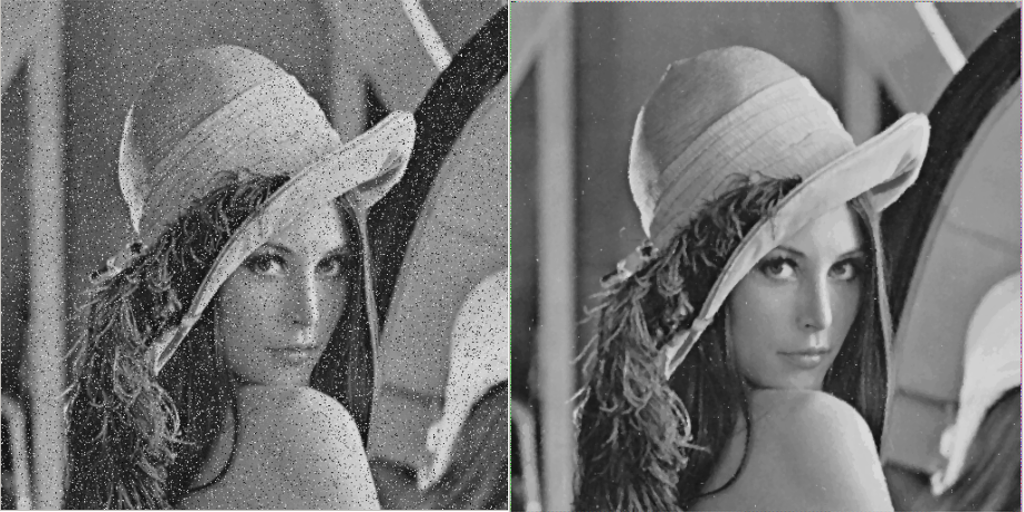
\includegraphics[width=0.6\textwidth]{median}
  \caption{Applying the Median filter to a noisy image of lena.}
\end{figure}

The width of the Median Filter can also be changed in the program. The interesting observation about this filter is that I used a Median Filter of width 3. If I use wider filters, the image will start to look like vector images and it starts to flatten out.

\begin{figure}[h!]
  \centering
    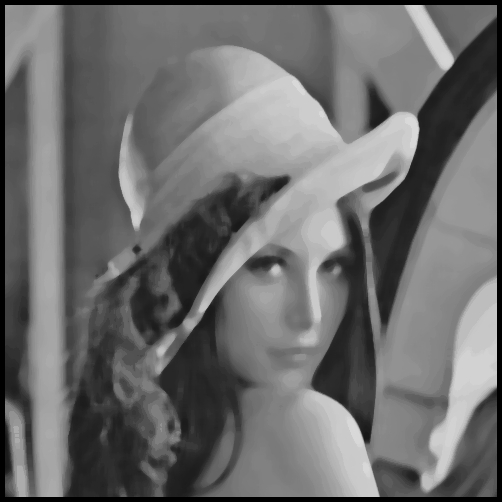
\includegraphics[width=0.3\textwidth]{big_median}
  \caption{Applying a 10x10 Median filter to the original image of lena.}
\end{figure}

\end{homeworkSection}

\end{homeworkProblem}

%----------------------------------------------------------------------------------------
%	Contrast Enhacement
%----------------------------------------------------------------------------------------

\begin{homeworkProblem}[\Roman{homeworkProblemCounter}. Contrast Enhancement]

As discussed in the class, the contrast of an image can be improved to a degree by stretching out the histogram to cover the whole space. To do this, first we need to find the dominant peak or peaks of the image. After finding the peak, we need to determine the valleys around the peak(s). The location of these valleys (we will have two valleys in this case, one on each side of the peak) can be used as stretching points of the histogram.

I have previously implemented a peak recognition system in a different context. In that method, first, I use a simple threshold (which can be determined using different statistical measures) to separate peak values from values located in valleys. After this step, I use Student T-test which is again another statistical test to figure out which peak is worth keeping and which peak is not. Also, using the resulting p-values from the T-test, I will decide whether I need to combine to consecutive peaks or treat them as separate peaks. This method has been implemented and is going to be published as an application note. But here, in our application, I just let the user to decide which two values he is going to use as the boundaries of the stretching process.

\begin{figure}[h!]
  \centering
    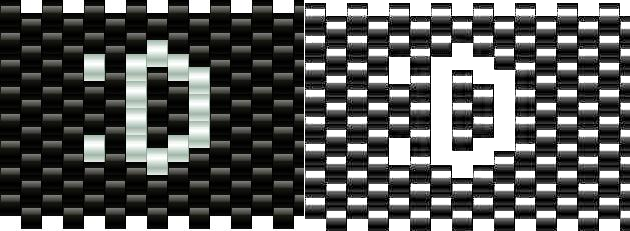
\includegraphics[width=0.6\textwidth]{enhance}
  \caption{This figure shows an image before and after the contrast enhancement process. The image on the left is the original image. The right image is the enhanced version.}
\end{figure}

\end{homeworkProblem}

%----------------------------------------------------------------------------------------
%	Thresholding
%----------------------------------------------------------------------------------------

\begin{homeworkProblem}[\Roman{homeworkProblemCounter}. Binarization an image]
As many other image processing techniques which don't have a unique way of doing, binarization of an image can also be done in many ways. Methods implemented in this project are,

\begin{enumerate} \itemsep1pt \parskip0pt \parsep0pt
  \item Simple Thresholding
  \item P-tile Thresholding
  \item Iterative Thresholding
  \item Adaptive Thresholding
  \item Slicing an image and do Thresholding
\end{enumerate}

In the following sub-sections I will present the results from running these techniques on different images and will briefly discuss each one of them.

\begin{homeworkSection}{(a) Simple Thresholding} % Section within problem

A simple threshold will be used in this technique and simply turns all the pixels below that threshold to black and the others to white. An example of this technique can be seen in the following figure,

\begin{figure}[h!]
  \centering
    
\includegraphics[width=0.6\textwidth]{simple_t}
  \caption{Applying a simple threshold to an image.}
\end{figure}

The user can define the threshold he wants to use using a slide control which starts from 0 and ends at 255.

\end{homeworkSection}

\begin{homeworkSection}{(b) P-Tile Thresholding} % Section within problem

In this method, we get the \textit{P} value and use it to find the \textit{Pth} percentile of the pixels. This percentile value can be used as an threshold value to convert the image to binary. An example of this method can be used which is done with \textit{P = 20}.

\begin{figure}[h!]
  \centering
    
\includegraphics[width=0.6\textwidth]{p_tile}
  \caption{Applying a P-tile function with \textit{P = 20}.}
\end{figure}

\end{homeworkSection}

\begin{homeworkSection}{(c) Iterative Thresholding} % Section within problem

This is just the implementation of the Iterative method discussed in the class. It doesn't need any input parameters and I will use 128 as the initial threshold value. The resulting image after applying this function on lena's image is depicted in the following figure.

\begin{figure}[h!]
  \centering
    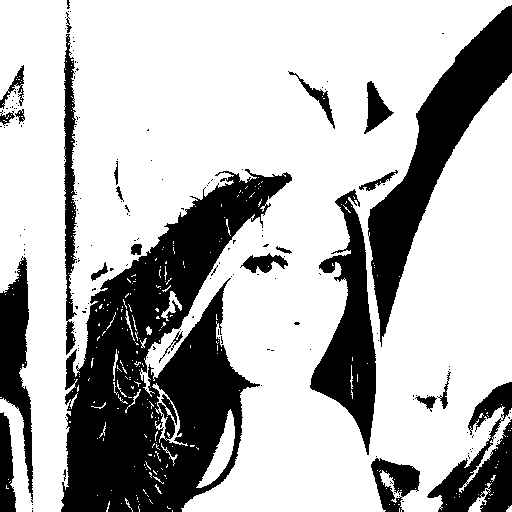
\includegraphics[width=0.3\textwidth]{iterative}
  \caption{Result of Iterative Thresholding on lena's image.}
\end{figure}

\end{homeworkSection}

\begin{homeworkSection}{(d) Adaptive Thresholding} % Section within problem

Adaptive thresholding will cut the image into N * N smaller images and will apply an arbitrary thresholding techniques on each one these smaller images individually. In my program, I get the number of images in each dimension, cut the image into smaller ones and apply an Iterative thresholding technique on each one of them and stitch them back together at the end. The resulting image from the lena's picture can be seen in the following figure in which I will cut the image into 10 smaller images on each dimension which will give us 100 separate images.

\begin{figure}[h!]
  \centering
    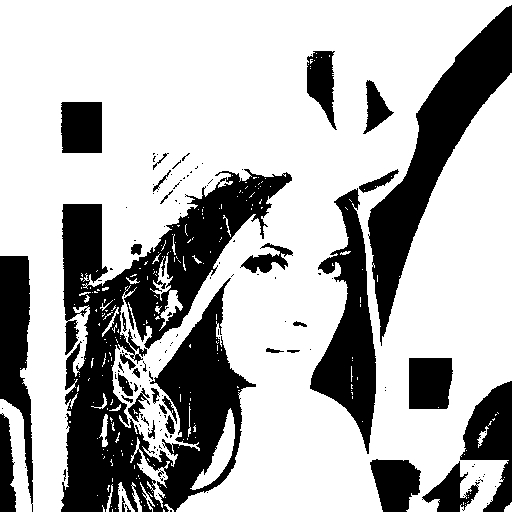
\includegraphics[width=0.3\textwidth]{adaptive}
  \caption{Result of Adaptive Thresholding on lena's image with 10 images on each dimension.}
\end{figure}

\end{homeworkSection}

\begin{homeworkSection}{(e) Image Slicing} % Section within problem

This technique can also be done in many different ways. In this project, I decided to slice the histogram into \textbf{N} equal areas. For each one of these areas, the values located inside of the area will be shown white and the rest of the pixels will be shown black.

After calculating the results, a new window will appear, showing the resulting images as an animation which plays twice. Also, the program will ask for a location to save all the results in case you want to review the results individually.

The following figure shows a image sliced into five different binary images.

\begin{figure}[h!]
  \centering
    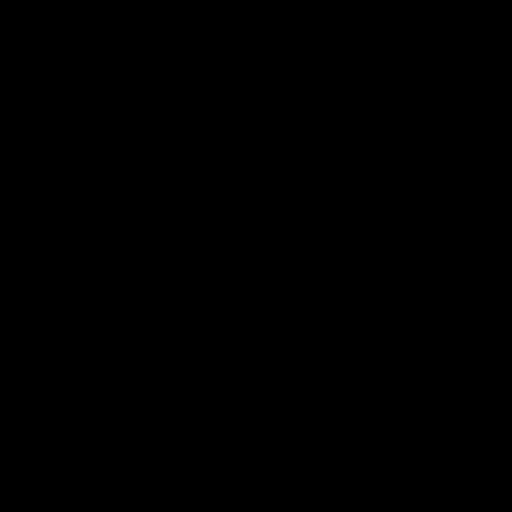
\includegraphics[width=0.3\textwidth]{slice1}
    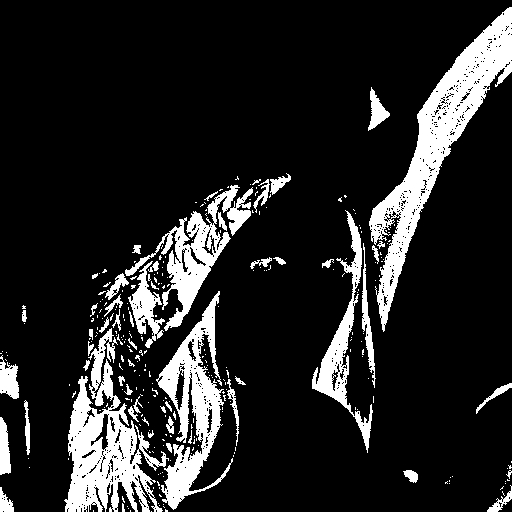
\includegraphics[width=0.3\textwidth]{slice2}
    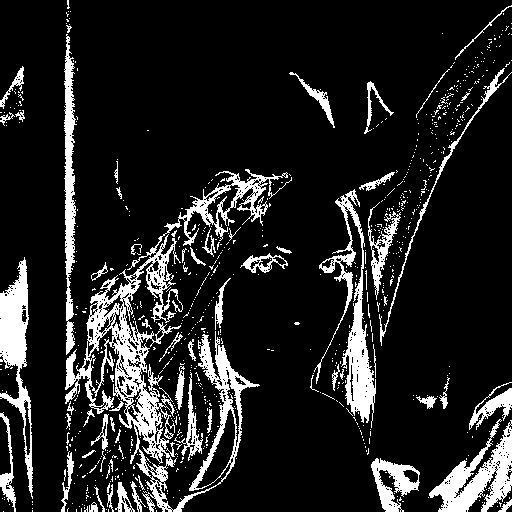
\includegraphics[width=0.3\textwidth]{slice3}
    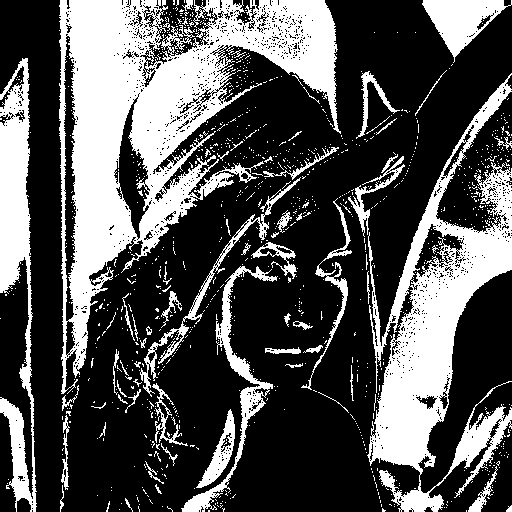
\includegraphics[width=0.3\textwidth]{slice4}
    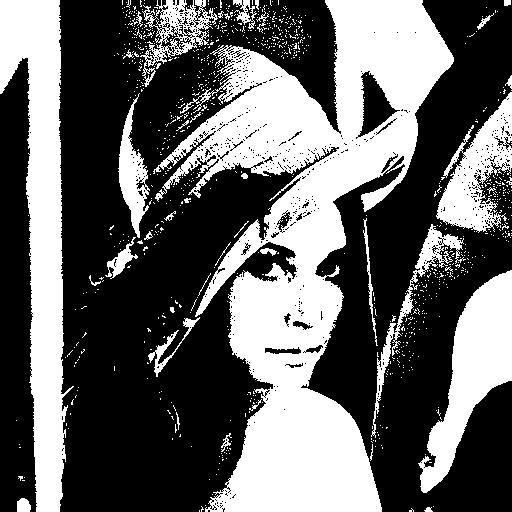
\includegraphics[width=0.3\textwidth]{slice5}
  \caption{Lena's image sliced into 5 different binary images. The histogram is sliced from left to right in which the top-left image will corresponds to the left most slice of the histogram.}
\end{figure}

\end{homeworkSection}

\end{homeworkProblem}

%----------------------------------------------------------------------------------------
%	Conclusion
%----------------------------------------------------------------------------------------

\begin{homeworkProblem}[\Roman{homeworkProblemCounter}. Contrast Enhancement]
As you may have figured out, Image Processing operations can be done in many different ways with many different parameters. Deciding on which technique to use and what parameters to use depends heavily on the application domain you are working in.


\end{homeworkProblem}

\end{document}
